% !TeX root = ../notes.tex

\section{Introduction}
Queries involve multiple steps to be performed. All techniques obviously depend on the physical characteristic of hardware, however there are algorithms and data structures able to help making them faster.

Query optimization is specifically important since SQL-like languages are declarative, hence do not specify the exact computation. Furthermore, the same query can be performed in multiple ways, and choosing the correct one is not trivial (depending on size, indices and more).

For instance, looking at cardinality of joins can either cause a Cartesian product of a hundred or several thousands, depending on the order in which they are executed. Often the human-written sequential order of instructions is not the most efficient one.

\subsection{Query Processing}
Query processing consists in: 
\begin{enumerate}
	\item Taking a text query as input;
	\item Compiling and optimizing;
	\item Extract the execution plan;
	\item Executing the query.
\end{enumerate}
Roughly, it can ve differentiated between compile time and runtime system. Most systems strongly separate those phases, for example using so-called prepared queries.
\begin{lstlisting}[language=SQL]
SELECT S.NAME
FROM STUDENTS S
WHERE S.ID = ?
\end{lstlisting}
Compilation takes time and limits the number of queries which can be ran in parallel. This kind of query can be executed over and over providing a value \texttt{Q1(123)} without the compilation overhead.

Embedded SQL is another technique to optimize compilation time in the case of large periods of time between the two phases. The programming language compiler takes care of the SQL part as well, optimizing it.

Specifically, the steps executed in compile time are:
\begin{enumerate}
	\item Parsing, AST production (abstract syntax to understand the structure);
	\item Schema lookup, variable binding, type inference (semantic analysis about relations and columns, syntax check);
	\item Normalization, factorization (bringing the query in abstract form, avoiding computing the same thing twice, evaluating expressions);
	\item Unnesting, deriving predicates, resolution of views (the plan generator can finally construct a cost-based model);
	\item Construction of execution plan;
	\item Review, pushing joins and refining the plan in general;
	\item Production of imperative plan (code generation).
\end{enumerate}
Rewrite I involves steps 1-3, while 4 and 5 compose rewrite II.

Example (with views):
\begin{lstlisting}[language=SQL]
SELECT name, salary
FROM employee, department
WHERE dep = did
AND location = "Munich"
AND area = "Research"
\end{lstlisting}

\begin{figure}[h]
	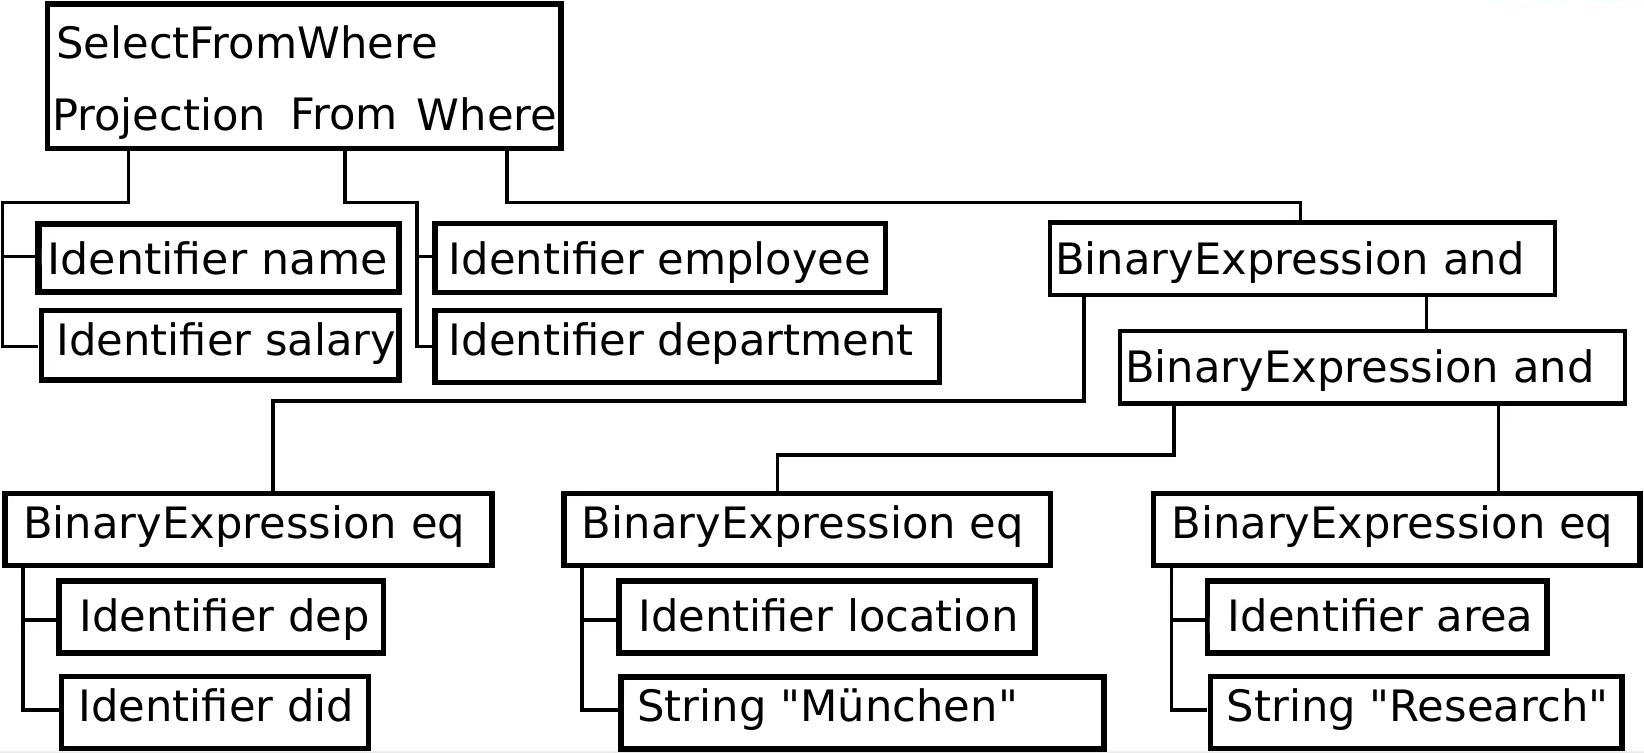
\includegraphics[scale=1.1]{query_plan.png}
	\centering
\end{figure}
Finally, the execution tree is built and polished, with the join operation on top and selects on nodes, reducing the amount of tuples to be joined. In other cases, such as regular expressions which are hard to evaluate, filtering can be done later.

The executable plan is a set of tuples containing variables or constants along and their type, with the main function loading query parameters, operations and allocated resources. 

Usually query planners are much more complicated and have practical difficulties: for instance, a long list of AND/OR predicates (machine-generated in the order of hundreds of thousands) can make the binary tree recursion crash due to insufficient space in the stack.

\subsection{Query Optimization}
Possible goals of query optimization include minimizing response time, resource consumption, time to first tuple (producing the first tuple as quick as possible, for instance with search results) or maximizing throughput. This can be expressed as a cost function: most systems aim to minimize response time, having resources as constraints.

Algebraic optimization is a branch using relational algebra to find the cheapest expression equivalent to the original. However, finding the cheapest is a practically impossible problem: it is hard to test for equivalence (numerical overflow, undecidable), the set of expressions is potentially huge and some algorithms are NP-hard (actual search space is limited and smaller than the potential one). 

There are ways to transform numerical expressions in algebraic ones, yet they might be expensive: calculus is faster to evaluate than algebra. 

Optimization approaches can be:
\begin{itemize}
	\item Transformative, taking an algebraic expression and iteratively making small changes, not efficient in practice;
	\item Constructing, starting from small expressions and joining them, obtaining larger sets, usually the preferred approach.
\end{itemize}

\subsection{Query Execution}
Query execution is the last step, the one directly benefiting from optimization. In reality, operators can perform extremely specialized operations, treating data as bags (sets with duplicates) or streams.




